\documentclass[11pt]{article}

\usepackage[utf8]{inputenc}
\usepackage{amsmath}
\usepackage{amssymb}
\usepackage{geometry}
\usepackage{graphicx}
\usepackage{booktabs}
\usepackage{float}

\geometry{margin=1in}

\title{Constraint-Preserving PINNs for Lindblad Quantum Dynamics}

\author{Nathan Hangen \\ Department of Physics \\ Wright State University}

\date{}

\begin{document}

\maketitle

\begin{abstract}

Physics-informed neural networks (PINNs) have emerged as powerful tools for modeling physical systems by embedding differential equations within neural architectures.
However, quantum systems impose strict physical constraints: density matrices must remain Hermitian, positive semidefinite, and trace normalized. 
Standard PINN approaches enforce these constraints through penalty terms in the loss function, which does not guarantee physical validity.

We introduce a constraint-preserving PINN architecture that guarantees quantum state validity by construction using a trace-normalized Gram matrix parameterization. 
This removes entire categories of failure seen in penalty-based approaches and produces stable training across repeated runs. 
Across 100 independent training trials our model achieved a 99\% success rate under explicitly defined physical validity criteria, while a penalty-based baseline succeeded in 67\% of trials.

We further introduce a quantum hardware validation pipeline using IBM quantum processors. 
A discrepancy between PINN predictions and hardware measurements revealed an initial-condition mismatch and highlighted the role of stationary states in Lindblad dynamics. 
Hardware validation therefore functions as a diagnostic tool for identifying modeling inconsistencies. 
Our results provide a framework for combining physics-informed machine learning with experimental quantum systems.
We also characterize spectral bias in density-matrix PINNs and provide a frequency-domain supplement.

\end{abstract}

\section{Introduction}

Physics-informed neural networks (PINNs) integrate physical laws into machine learning by embedding governing differential equations into neural network training objectives \cite{raissi2019}. 
These methods have been successfully applied across scientific domains including fluid mechanics, materials science, and plasma physics.
Neural-network quantum states have also proven effective as compact variational representations for many-body wavefunctions, demonstrating high-accuracy ground-state and dynamical predictions \cite{carleo2016}.

Quantum systems introduce additional constraints beyond differential equations.
A valid quantum state must be represented by a density matrix $\rho$ satisfying

\begin{enumerate}
\item Hermiticity: $\rho = \rho^\dagger$
\item Positivity: $\rho \succeq 0$
\item Unit trace: $\mathrm{Tr}(\rho) = 1$
\end{enumerate}

Traditional PINN approaches attempt to enforce these constraints using penalty terms added to the training loss.
While such penalties reduce violations, they do not guarantee physical validity and often lead to unstable training or non-physical intermediate solutions.

We propose an alternative strategy: embedding these constraints directly into the neural architecture.
This guarantees that the model outputs remain physically valid throughout training and evaluation.
Recent work on deep PINNs highlights that architectural changes are often required to mitigate depth-related pathologies and unlock stable training behavior \cite{jiang2025deeperpinns}.

Additionally, we explore validation of neural physics models using real quantum hardware.
Rather than treating hardware comparisons purely as verification, we demonstrate that discrepancies between model predictions and hardware measurements can reveal modeling inconsistencies such as mismatched initial conditions or stationary states of the governing dynamics.

The baseline PINN used for comparison follows the standard approach in the physics-informed neural network literature, where density matrix elements are predicted directly and physical constraints are enforced through loss penalties rather than architectural guarantees.
This comparison is motivated in part by evidence that gradient-based training favors low-frequency functions, an implicit bias that can dominate learning dynamics in PINNs and promote overly smooth or stationary solutions \cite{rahaman2019,xu2018,arpit2017,neyshabur2014,zhang2017}.

\section{Quantum Dynamics Background}

\subsection{Density Matrices}

The state of a quantum system can be represented by a density matrix $\rho$ \cite{breuer2002}.
For a two-level system (qubit),

\begin{equation}
\rho =
\begin{pmatrix}
\rho_{00} & \rho_{01} \\
\rho_{10} & \rho_{11}
\end{pmatrix}
\label{densitymatrix}
\end{equation}

where diagonal elements represent populations and off-diagonal elements represent quantum coherences.

A physically valid density matrix must be Hermitian, positive semidefinite, and trace normalized.

\subsection{Lindblad Master Equation}

Open quantum system dynamics are governed by the Lindblad master equation \cite{lindblad1976,breuer2002}

\begin{equation}
\frac{d\rho}{dt}
=
-i[H,\rho]
+
L \rho L^\dagger
-
\frac{1}{2}
\{L^\dagger L,\rho\}
\label{lindblad}
\end{equation}

where $H$ is the system Hamiltonian, $L$ is the Lindblad operator describing dissipation, and $\sigma_x,\sigma_y,\sigma_z$ denote the Pauli operators. Here $[\cdot,\cdot]$ denotes a commutator and $\{\cdot,\cdot\}$ denotes an anticommutator.

For pure dephasing with $L = \sqrt{\gamma}\sigma_z$, the populations remain constant while the off-diagonal coherence decays exponentially.

Importantly, any density matrix diagonal in the $\sigma_z$ basis is stationary under pure dephasing dynamics.
For this case the dissipator generated by $L=\sqrt{\gamma}\sigma_z$ leaves all states diagonal in the $\sigma_z$ basis unchanged.
The maximally mixed state

\begin{equation}
\rho = \frac{I}{2}
\label{maxmixed}
\end{equation}

is therefore one member of a stationary manifold rather than a unique fixed point.

\section{Constraint-Preserving Neural Architecture}

\subsection{Architecture Overview}

Instead of directly predicting the entries of $\rho$, the network predicts parameters defining an auxiliary matrix $A(t)$.

The density matrix is then constructed as

\begin{equation}
\rho(t)
=
\frac{A(t)A^\dagger(t)}
{\mathrm{Tr}(A(t)A^\dagger(t))}
\label{gram}
\end{equation}

This construction guarantees

\begin{itemize}
\item Hermiticity
\item Positive semidefiniteness
\item Unit trace
\end{itemize}

because $AA^\dagger$ is a Gram matrix.

\paragraph{Theorem.}
For any complex matrix $A(t)$ with $\mathrm{Tr}(A(t)A^\dagger(t))>0$, the matrix defined in Eq.~(\ref{gram}) is Hermitian, positive semidefinite, and trace normalized.

\paragraph{Proof.}
$A(t)A^\dagger(t)$ is Hermitian and positive semidefinite as a Gram matrix. Division by the positive real scalar $\mathrm{Tr}(A(t)A^\dagger(t))$ preserves both properties and enforces unit trace.

\subsection{Parameterization}

We define

\begin{equation}
A(t)
=
\begin{pmatrix}
e^{\alpha_1(t)} & 0 \\
\beta(t)+i\gamma(t) & e^{\alpha_2(t)}
\end{pmatrix}
\label{paramA}
\end{equation}

The neural network predicts the real functions

\[
\alpha_1(t),\alpha_2(t),\beta(t),\gamma(t)
\]

This parameterization represents a log-Cholesky form which fixes gauge freedom under transformations $A \rightarrow AU$ for unitary $U$.
While Gram matrix and Cholesky-style constructions are standard tools for enforcing positive semidefiniteness \cite{horn1990}, our contribution is to integrate this constraint-preserving representation directly into a PINN for Lindblad quantum dynamics.

\subsection{Training Objective}

The model minimizes the Frobenius norm of the Lindblad residual

\begin{equation}
\mathcal{L}_{\mathrm{phys}}
=
\left\|
\frac{d\rho}{dt}
-
\mathcal{D}[\rho]
\right\|_F^2
\label{physloss}
\end{equation}

where $\mathcal{D}[\rho]$ denotes the Lindblad generator defined in Eq.~(\ref{lindblad}).

A weak entropy regularization term is also used

\begin{equation}
\mathcal{L}
=
\mathcal{L}_{\mathrm{phys}}
+
\lambda \,
\mathrm{Var}_{t \in T}
\left(
S(\rho(t))
\right)
\label{totalloss}
\end{equation}

where

\begin{equation}
S(\rho) = -\mathrm{Tr}(\rho \log \rho)
\label{entropy}
\end{equation}

is the von Neumann entropy and the variance is computed across the discrete training time grid $T$.
Empirically, this term reduced convergence to nearly stationary solutions and improved training stability in our experiments.

\subsection{Baseline Loss}

The baseline PINN uses direct prediction of density matrix entries with penalty terms enforcing constraints:
\begin{equation}
\mathcal{L}_{\mathrm{base}} =
\left\|\frac{d\rho}{dt} - \mathcal{D}[\rho]\right\|_F^2
+ \lambda_{\mathrm{H}}\|\rho-\rho^\dagger\|_F^2
+ \lambda_{\mathrm{T}}(\mathrm{Tr}(\rho)-1)^2
+ \lambda_{\mathrm{P}}\Phi(\rho).
\label{baseloss}
\end{equation}
The baseline PINN follows the standard penalty-based formulation used in prior physics-informed neural network approaches \cite{raissi2019,bondesan2022}. Here $\Phi(\rho)$ denotes a positivity penalty constructed from the negative part of the eigenvalue spectrum of $\rho$, and $\lambda_{\mathrm{H}},\lambda_{\mathrm{T}},\lambda_{\mathrm{P}}$ are tuned on validation runs.

\section{Experimental Setup}

We consider a single-qubit pure dephasing model with
\[
H = \omega \sigma_z,
\qquad
L = \sqrt{\gamma}\,\sigma_z,
\qquad
\rho(0) = |+\rangle\langle+|.
\]
Under this model the populations remain constant while the coherences decay exponentially.

Training used a four-layer multilayer perceptron with Tanh activations.
Physical time $\tau \in [0,T]$ is linearly mapped to a normalized network input
$t \in [-1,1]$; reported times refer to the physical scale $\tau$.
\begin{equation}
t = \frac{2\tau}{T} - 1
\label{timemap}
\end{equation}

Optimization was performed using Adam for 5000 epochs.

\begin{table}[H]
\centering
\begin{tabular}{lll}
\toprule
Parameter & Baseline PINN & Constraint-preserving PINN \\
\midrule
Architecture & 4 layer MLP & 4 layer MLP \\
Activation & Tanh & Tanh \\
Outputs & 8 matrix entries & 4 parameters \\
Epochs & 5000 & 5000 \\
Optimizer & Adam & Adam \\
Trials & 100 & 100 \\
\bottomrule
\end{tabular}
\caption{Training configuration}
\label{tab:training}
\end{table}

\section{Success Criteria}

A training run was classified as successful if

\begin{enumerate}
\item Trace error $|\mathrm{Tr}(\rho)-1| < 10^{-12}$
\item Minimum eigenvalue $\ge -10^{-10}$
\item Final Lindblad residual $< 10^{-5}$
\end{enumerate}

\section{Results}

Across 100 independent random seeds:

\begin{table}[H]
\centering
\begin{tabular}{lcc}
\toprule
Metric & Baseline PINN & Constraint-preserving PINN \\
\midrule
Success rate & 67\% & 99\% \\
Max trace error & $10^{-7}$ & $<10^{-15}$ \\
Negative eigenvalues & Observed in failed runs & None \\
Training stability & frequent failed runs & stable across seeds \\
\bottomrule
\end{tabular}
\caption{Training outcomes across trials}
\label{tab:results}
\end{table}

\section{Spectral Bias Analysis}

To characterize frequency-dependent learning behavior, we performed a spectral analysis of the learned density-matrix trajectories.
We computed Fourier-domain errors between each model's predicted $\rho(t)$ and a numerical Lindblad reference solution under the same Hamiltonian and dissipator.
For each configuration we tracked low- and high-frequency error components across training epochs.
This analysis follows the spectral-bias framework that shows neural networks tend to learn low-frequency components faster than high-frequency components \cite{rahaman2019,xu2018}.

Figure~\ref{fig:spectral_error} shows that both the baseline and constraint-preserving PINN exhibit a pronounced low-frequency learning advantage: low-frequency error decreases rapidly while high-frequency error decays more slowly.
Increasing depth and width changes absolute error levels but does not eliminate the bias.
Figure~\ref{fig:spectral_spectrum} compares the final learned spectra to the Lindblad reference, highlighting residual high-frequency discrepancies even when fidelity is high.

\begin{figure}[H]
\centering
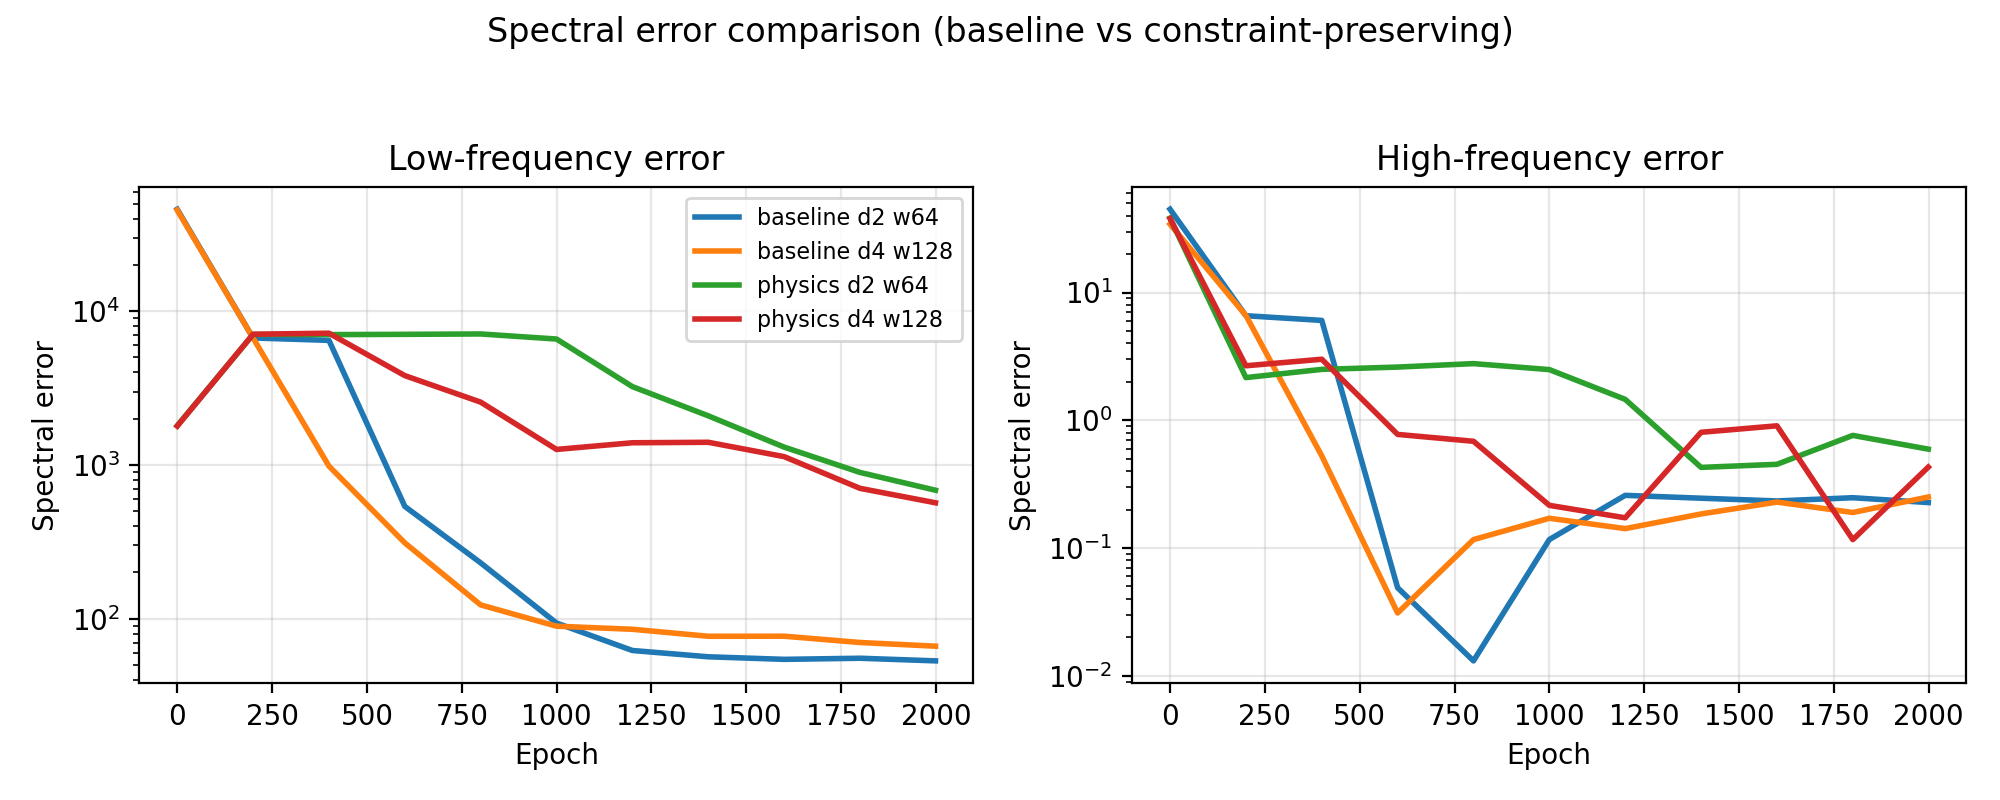
\includegraphics[width=0.9\linewidth]{figures/spectral_bias/spectral_error_comparison.png}
\caption{Low- and high-frequency error components during training for baseline and constraint-preserving PINNs (2x2 system). Both exhibit spectral bias: low-frequency error collapses faster than high-frequency error.}
\label{fig:spectral_error}
\end{figure}

\begin{figure}[H]
\centering
\begin{minipage}{0.48\linewidth}
\centering
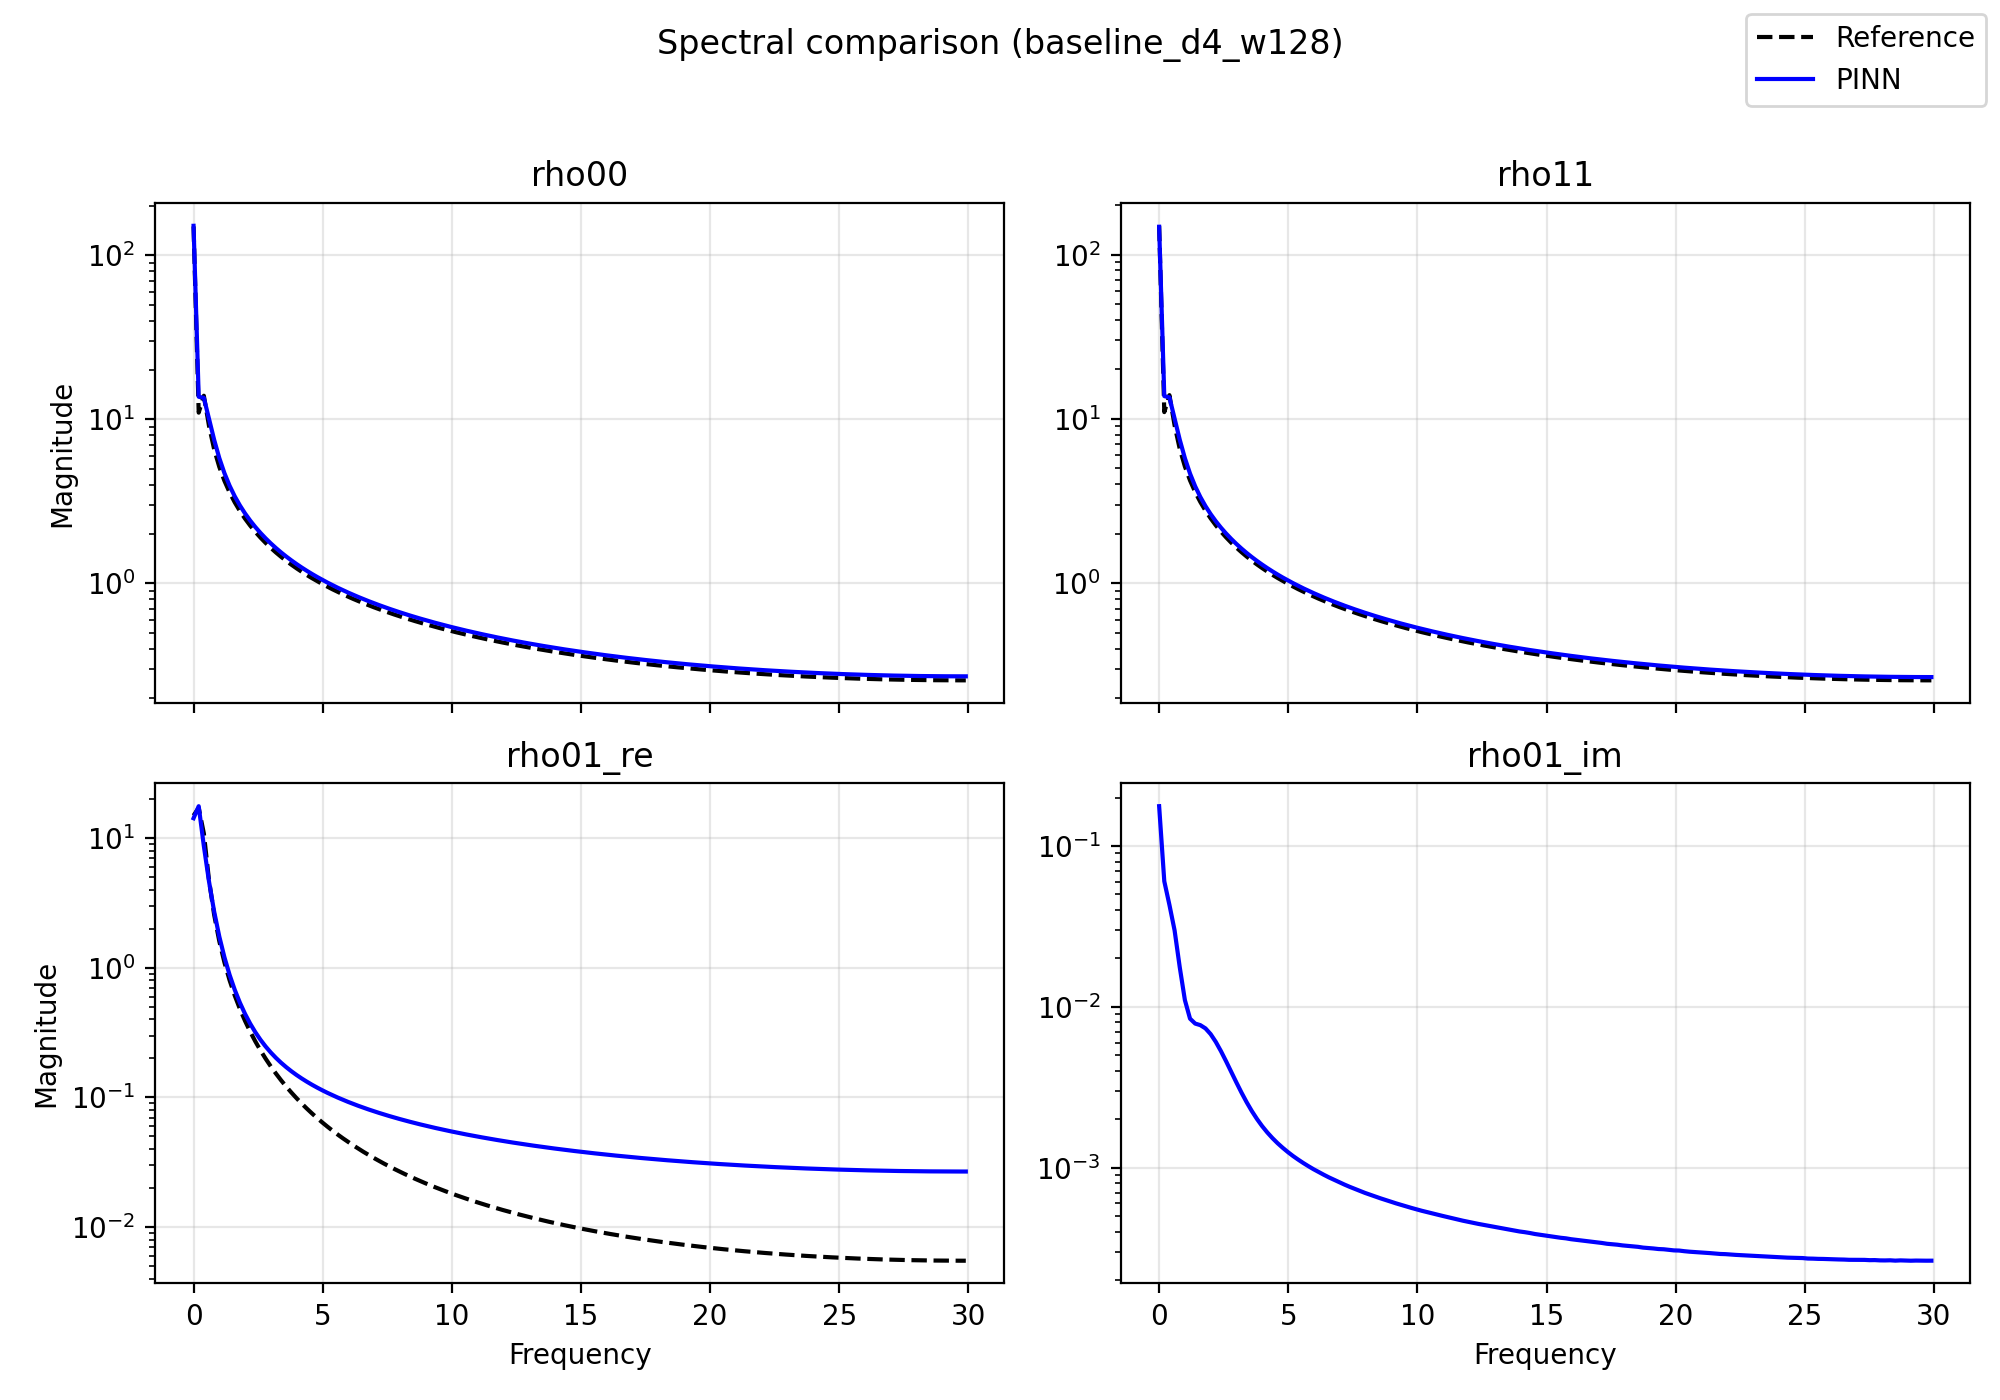
\includegraphics[width=\linewidth]{figures/spectral_bias/baseline_d4_w128_spectrum_comparison.png}
\caption*{Baseline PINN}
\end{minipage}
\hfill
\begin{minipage}{0.48\linewidth}
\centering
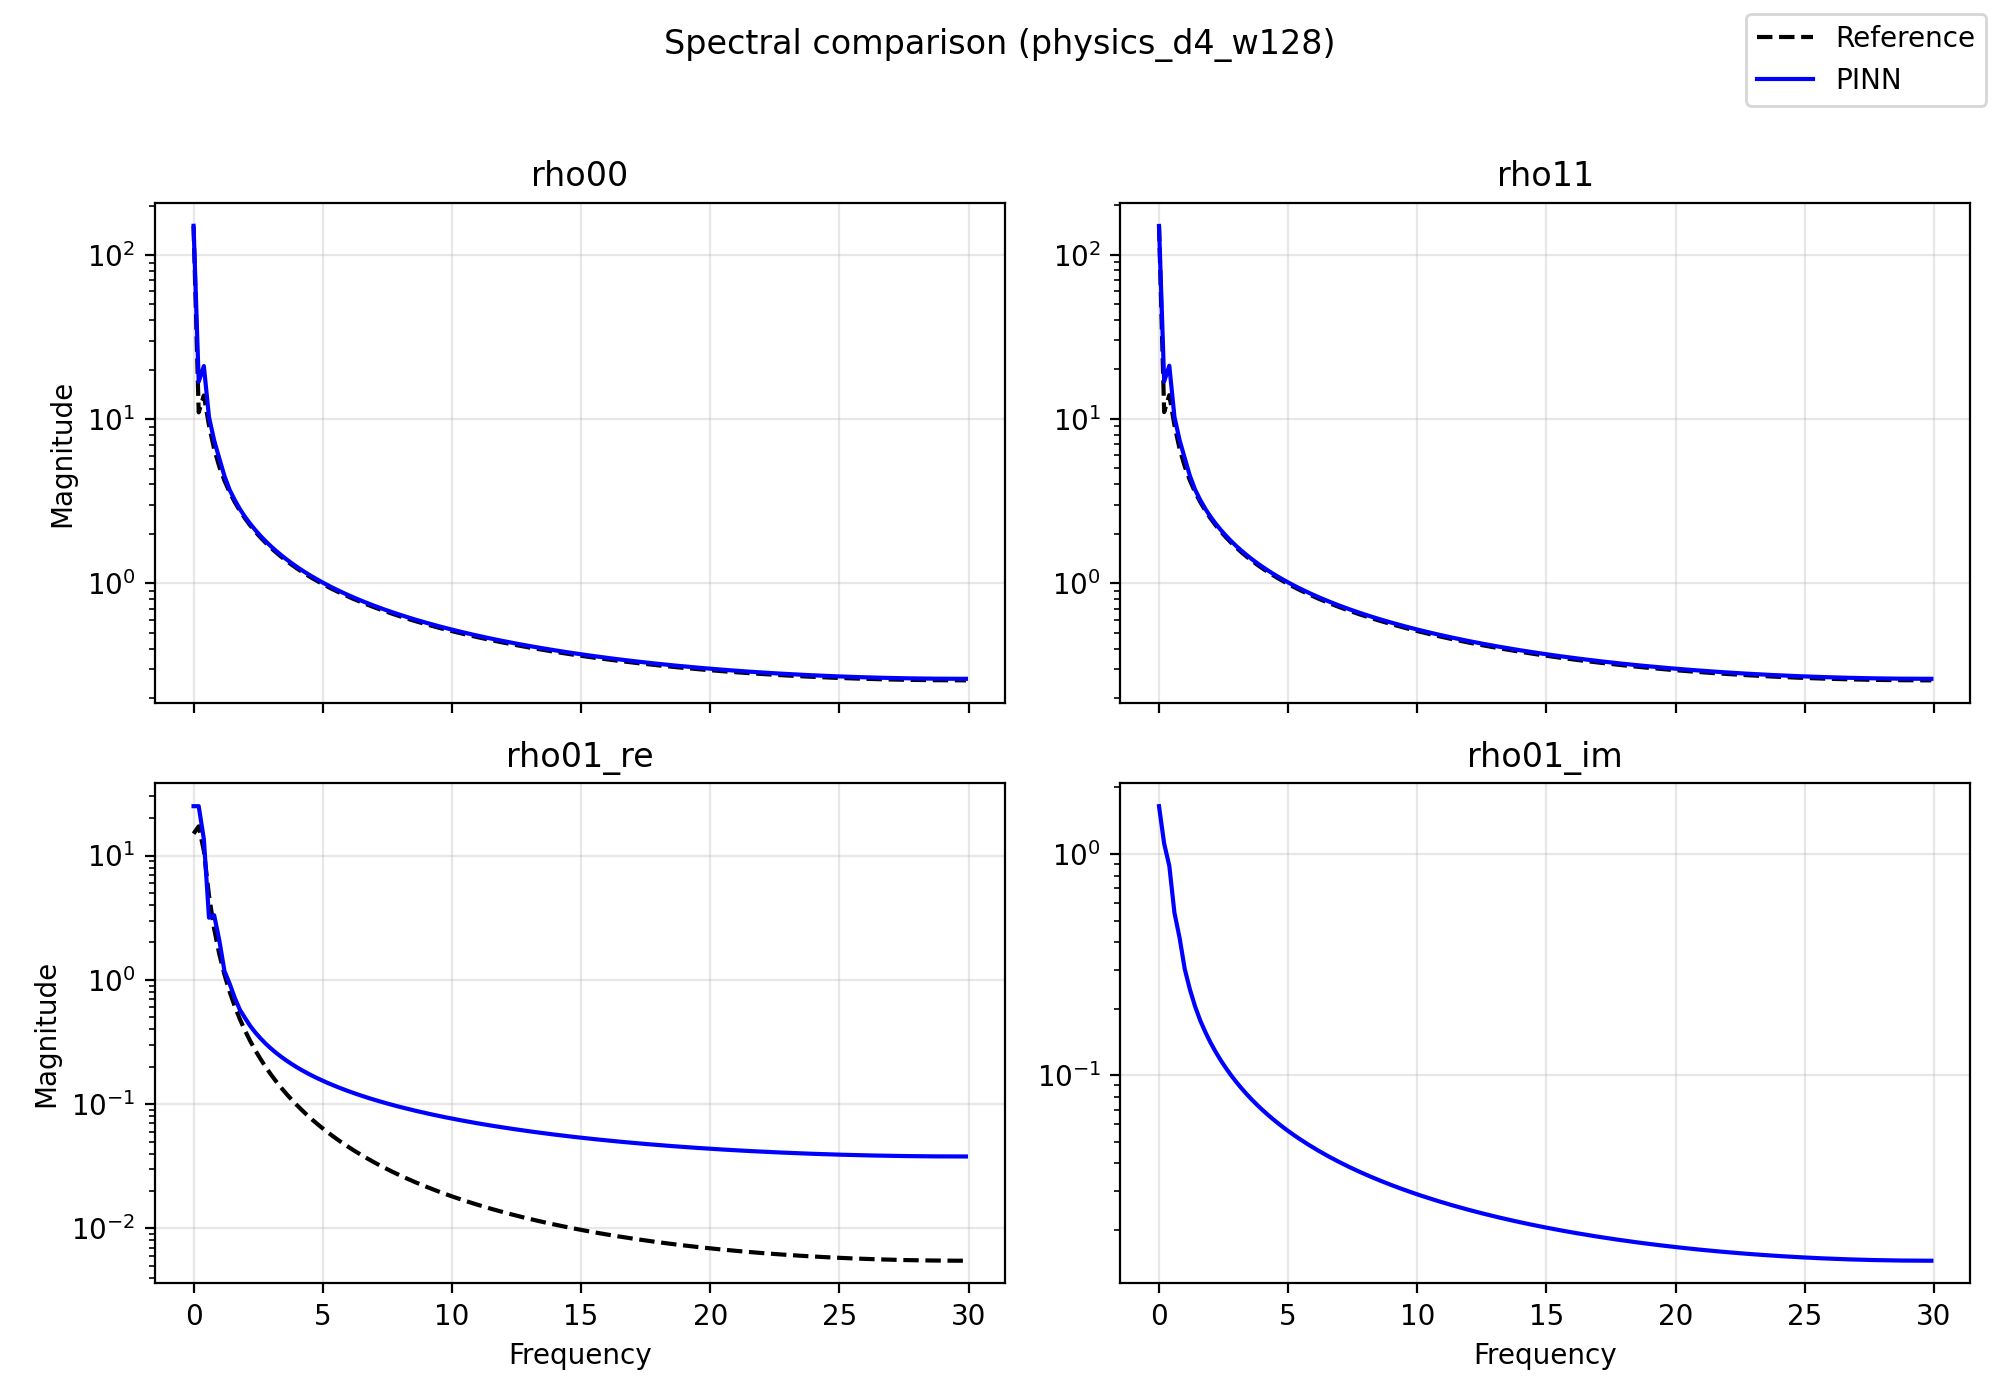
\includegraphics[width=\linewidth]{figures/spectral_bias/physics_d4_w128_spectrum_comparison.png}
\caption*{Constraint-preserving PINN}
\end{minipage}
\caption{Fourier magnitude spectra of density-matrix elements at final epoch versus the Lindblad reference for depth-4, width-128 models. High-frequency discrepancies persist even when overall fidelity is strong.}
\label{fig:spectral_spectrum}
\end{figure}

\section{Gradient Pathology Diagnostics}

We also quantified gradient imbalances across the composite loss terms that arise in penalty-based PINNs.
This follows prior work showing that stiff gradient flow can cause unbalanced gradients between physics residuals and constraint terms, destabilizing training \cite{wang2020gradient}.
Figure~\ref{fig:grad_pathology} shows per-term gradient norms for the baseline and constraint-preserving PINN.
In the baseline model, constraint penalties and physics residuals can differ by orders of magnitude, while the constraint-preserving PINN exhibits a simpler gradient structure dominated by the physics residual.

\begin{figure}[H]
\centering
\begin{minipage}{0.48\linewidth}
\centering
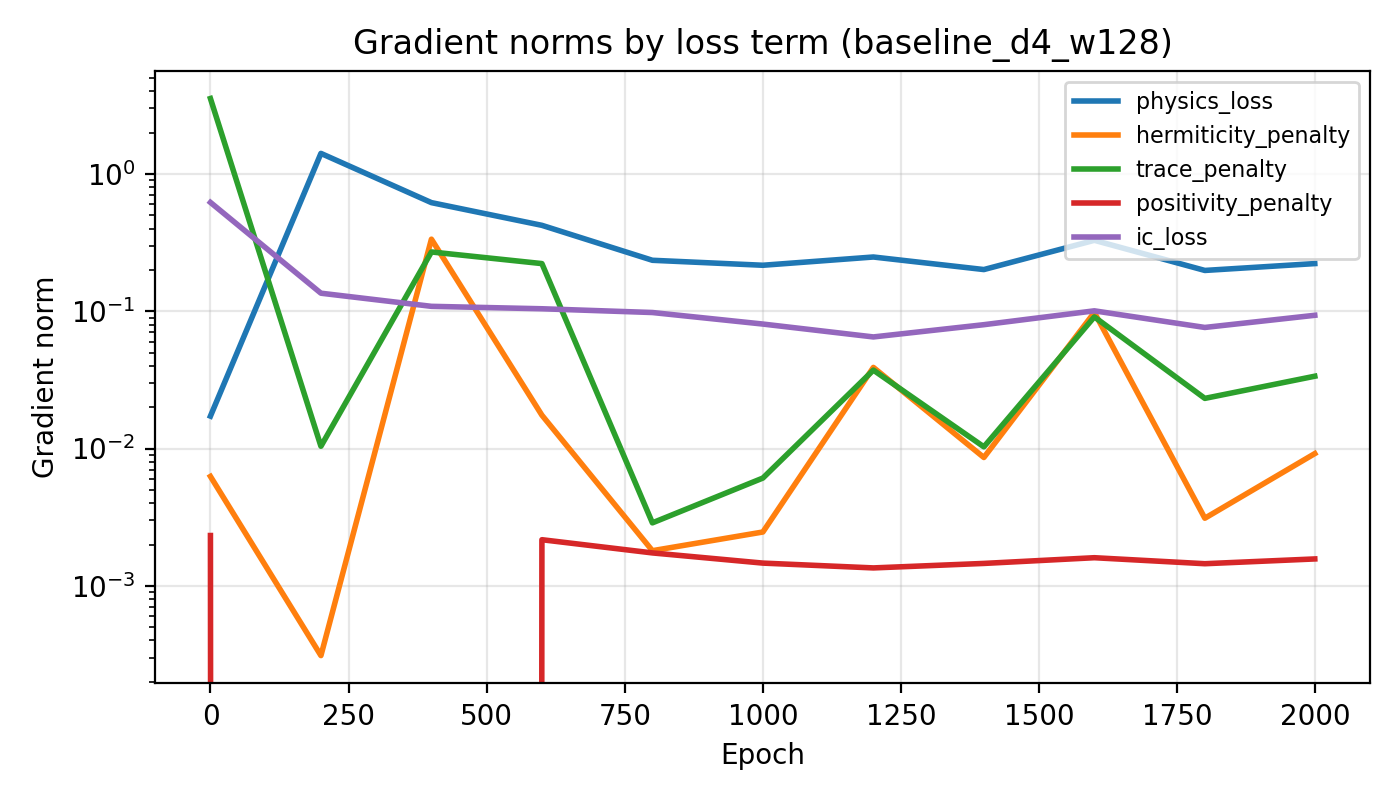
\includegraphics[width=\linewidth]{figures/spectral_bias/baseline_d4_w128_gradient_norms.png}
\caption*{Baseline PINN}
\end{minipage}
\hfill
\begin{minipage}{0.48\linewidth}
\centering
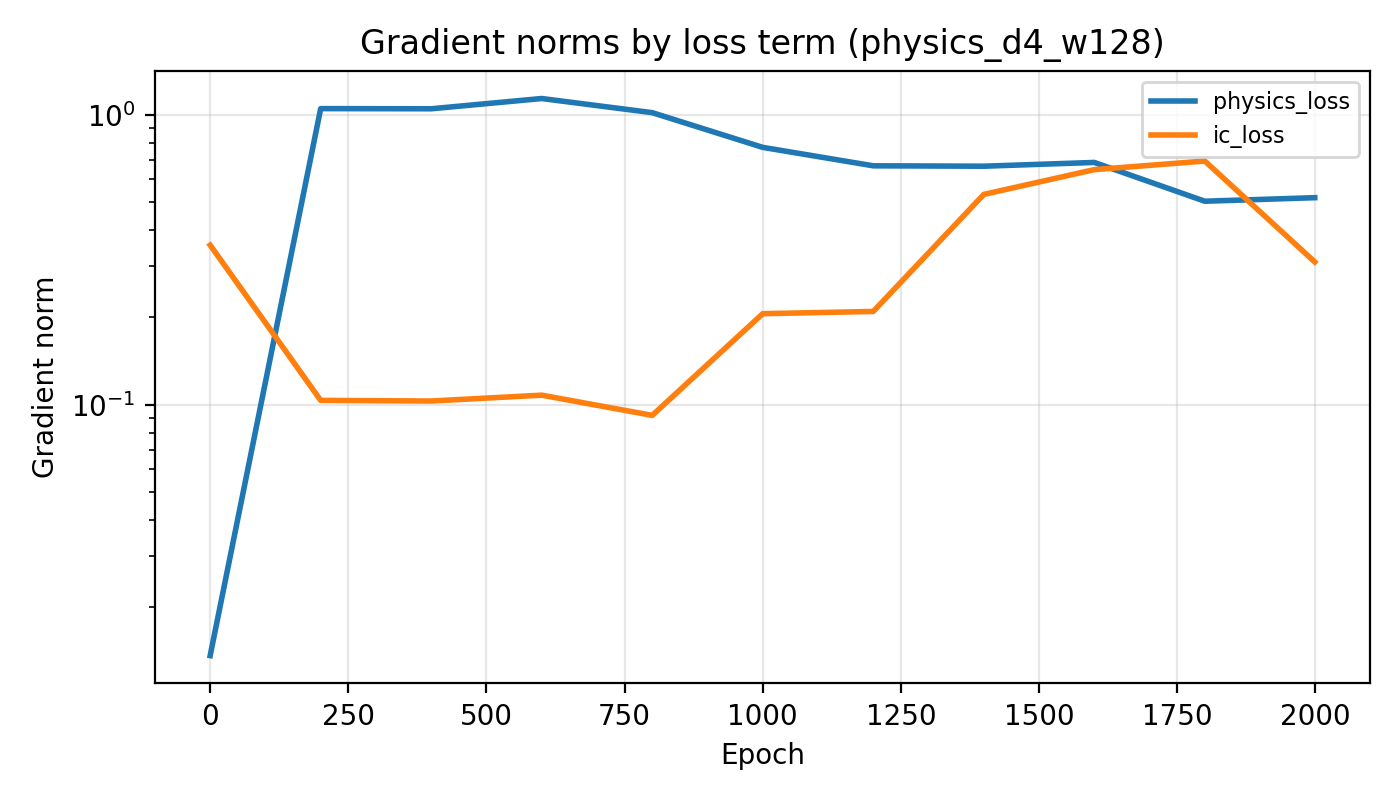
\includegraphics[width=\linewidth]{figures/spectral_bias/physics_d4_w128_gradient_norms.png}
\caption*{Constraint-preserving PINN}
\end{minipage}
\caption{Gradient norms by loss term for depth-4, width-128 models. Baseline training shows multi-term gradient imbalance; the constraint-preserving model reduces competing gradient scales.}
\label{fig:grad_pathology}
\end{figure}

\section{Depth Sweep}

Motivated by evidence that deep PINNs can degrade without architectural modifications \cite{jiang2025deeperpinns}, we performed a refined depth sweep (3000 epochs, 600 time points, three seeds per depth) using the constraint-preserving architecture. Depth increases consistently reduced the final loss but produced only marginal changes in mean fidelity, indicating that depth alone does not resolve the remaining accuracy gap. Figure~\ref{fig:depth_sweep_fidelity} summarizes fidelity versus depth for the refined sweep.

\begin{figure}[H]
\centering
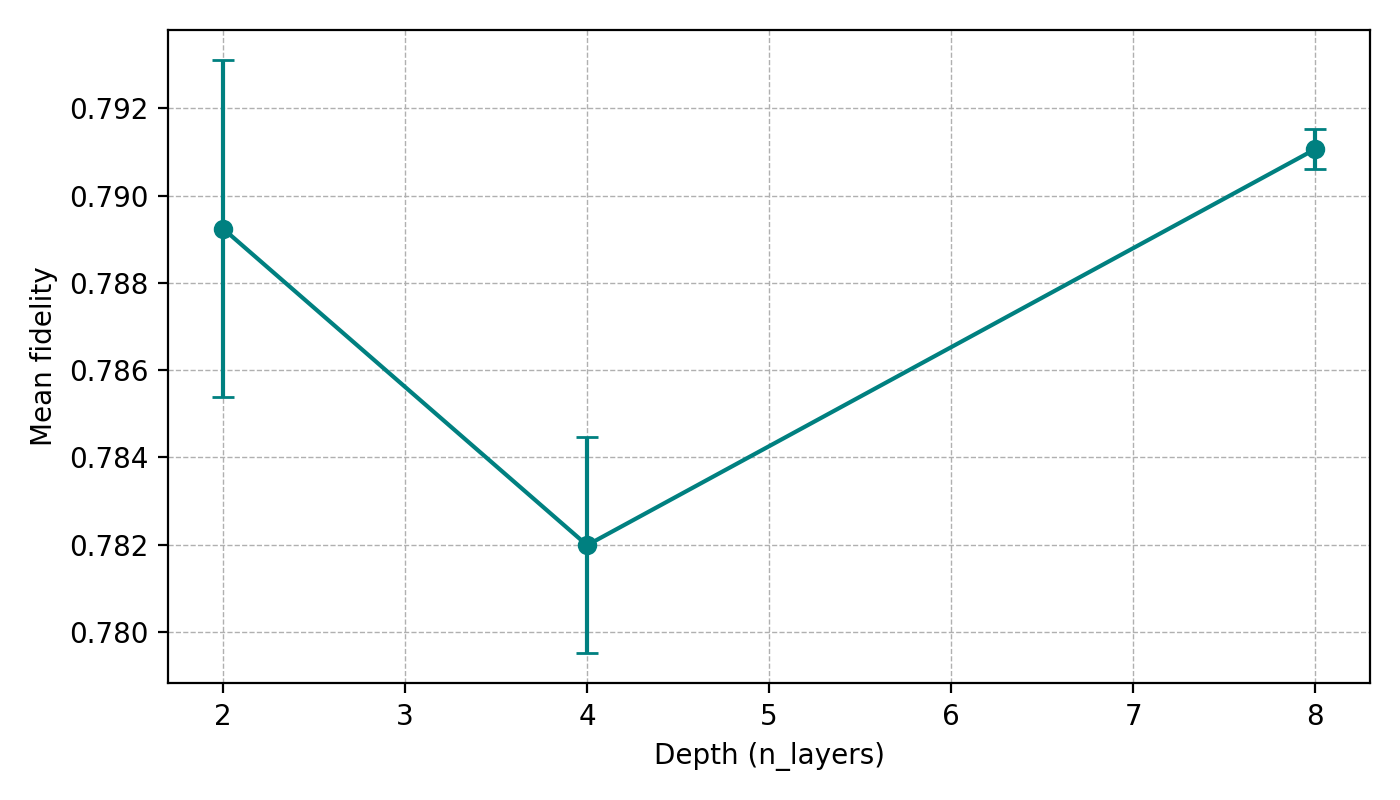
\includegraphics[width=0.75\linewidth]{figures/depth_sweep_refined/depth_sweep_refined_fidelity.png}
\caption{Mean fidelity versus depth for the refined sweep (3 seeds per depth, 3000 epochs, 600 time points). Fidelity plateaus across depths despite lower final losses at higher depth.}
\label{fig:depth_sweep_fidelity}
\end{figure}

\section{Architecture-Constrained Precedent}

Prior work on analytic constraints in neural emulators demonstrates that architectural enforcement can satisfy conservation laws to machine precision and improve constraint-sensitive outputs without degrading overall accuracy \cite{beucler2021}.
To align with this framing, we compare unconstrained (UC), loss-constrained (LC), and architecture-constrained (AC) variants on the same Lindblad task.
Figure~\ref{fig:constraint_compare} shows that the unconstrained model violates physical constraints, while the penalty-based baseline reduces but does not eliminate violations, and the constraint-preserving PINN maintains consistency.

\begin{figure}[H]
\centering
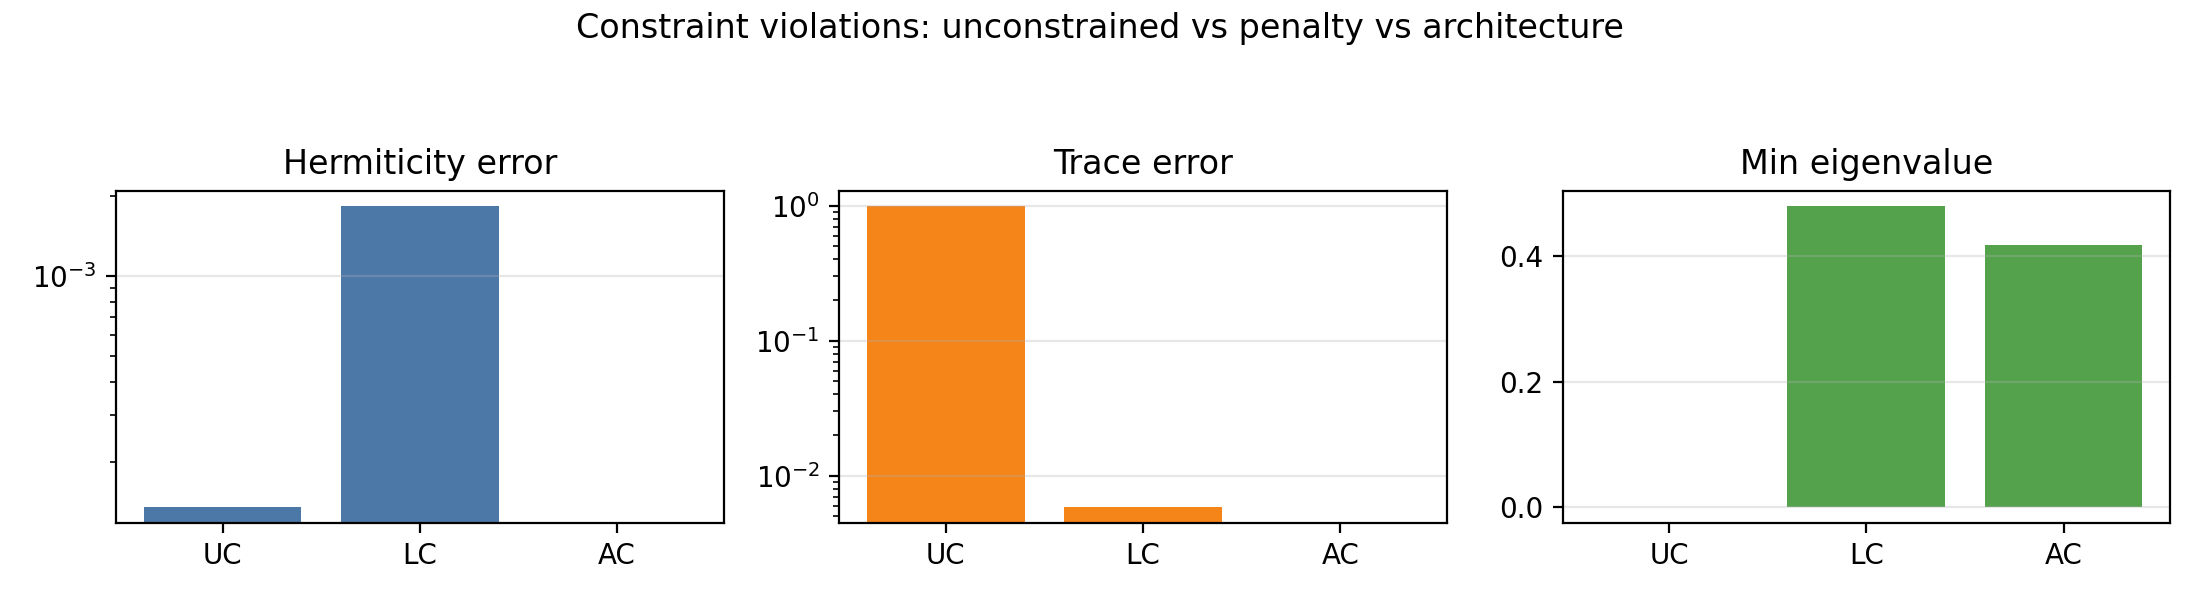
\includegraphics[width=0.9\linewidth]{figures/spectral_bias/constraint_violation_comparison.png}
\caption{Constraint violation comparison for UC (unconstrained), LC (loss-constrained baseline), and AC (architecture-constrained) models.}
\label{fig:constraint_compare}
\end{figure}

\begin{figure}[H]
\centering
\begin{minipage}{0.48\textwidth}
\centering
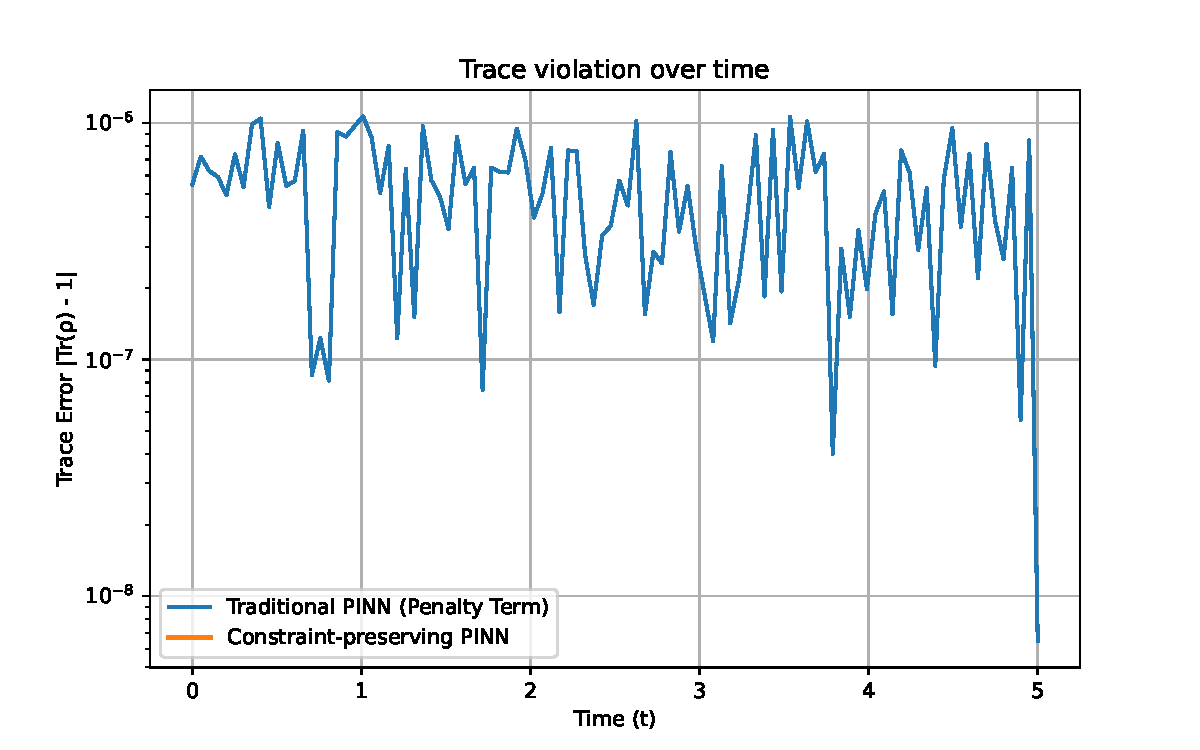
\includegraphics[width=\linewidth]{figures/fig_constraint_violation.pdf}
\end{minipage}
\hfill
\begin{minipage}{0.48\textwidth}
\centering
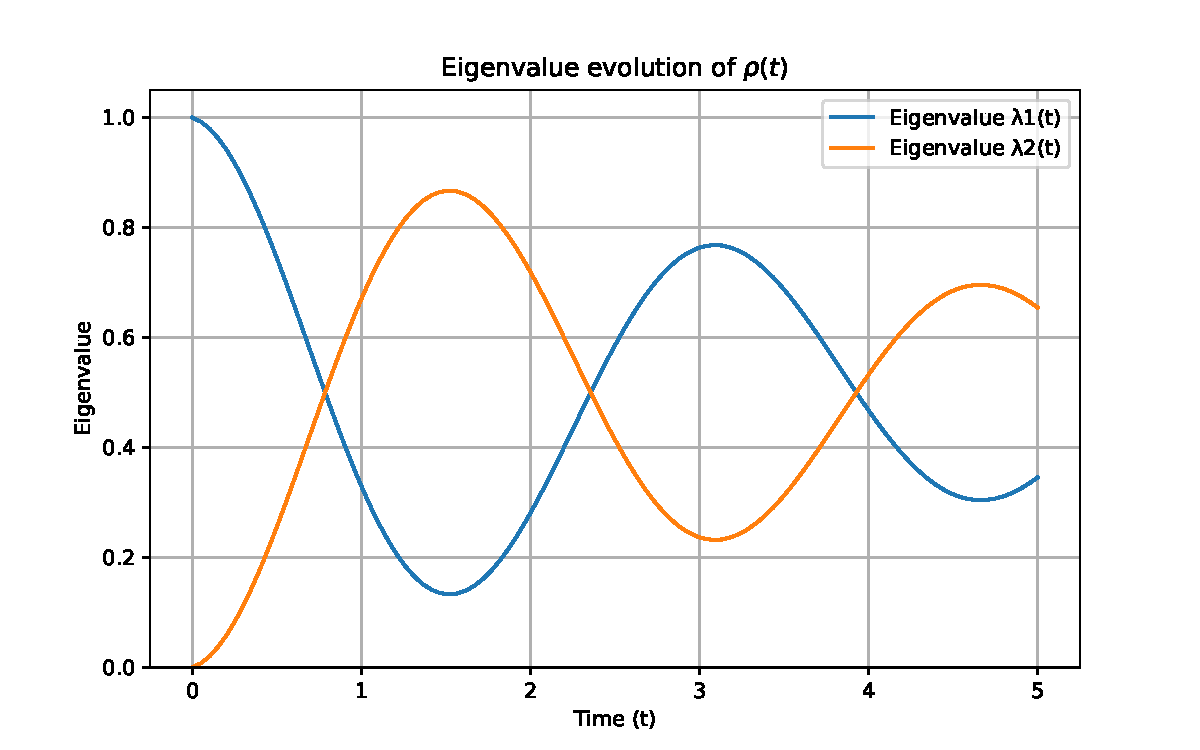
\includegraphics[width=\linewidth]{figures/fig_eigenvalue_evolution.pdf}
\end{minipage}
\caption{Constraint preservation versus baseline. Left: trace constraint violations. Right: minimum eigenvalue evolution highlighting positivity failures in the baseline.}
\label{fig:constraints}
\end{figure}

\begin{figure}[H]
\centering
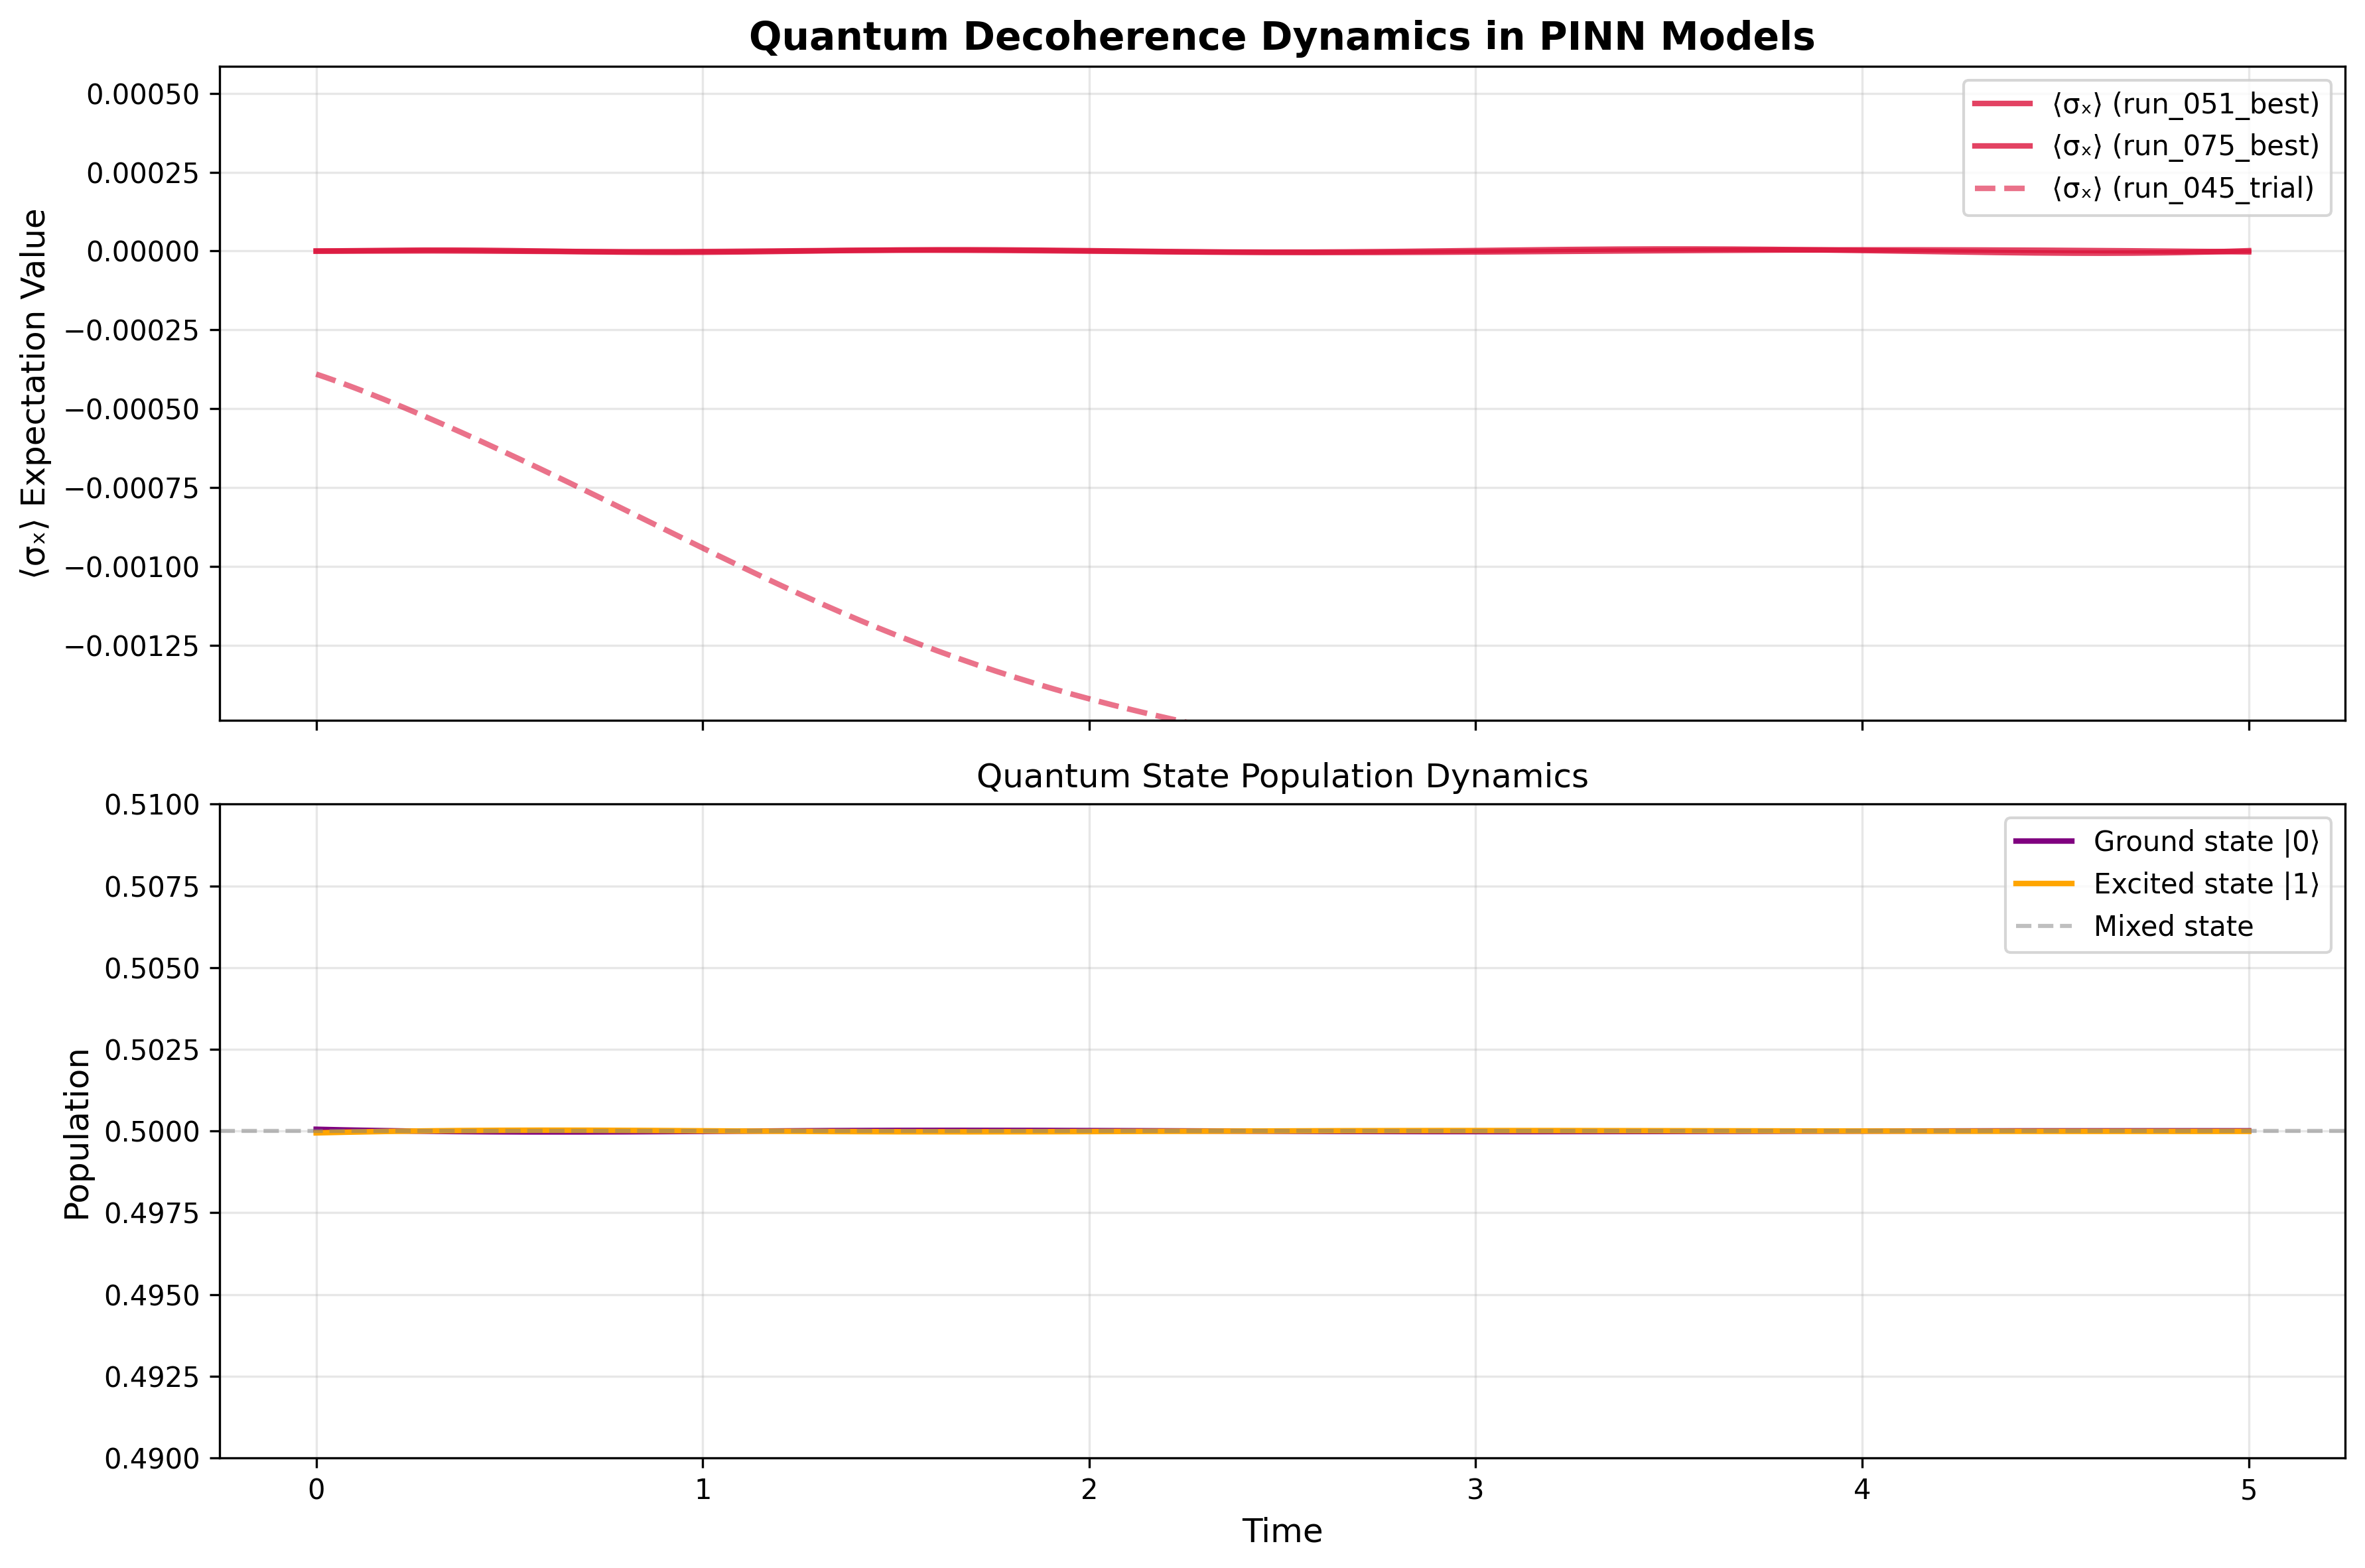
\includegraphics[width=0.75\textwidth]{figures/fig_dynamics.png}
\caption{Learned dynamics for the trained model. Populations remain stable while coherence decays under pure dephasing.}
\label{fig:dynamics}
\end{figure}

\section{Hardware Validation Pipeline}

To compare model predictions with physical experiments we developed a validation pipeline using IBM quantum hardware.
This hardware protocol is used as a diagnostic consistency check for stationary dephasing behavior, not as a direct validation of the $|+\rangle\langle+|$ initial-condition experiment used in training.

The hardware preparation approximates a maximally mixed state by executing circuits initialized to $|0\rangle$ and $|1\rangle$ with equal probability and averaging measurement results.
This is deliberately distinct from the model initial condition and is used to probe stationary behavior under dephasing.

Quantum evolution is implemented using a stochastic Pauli-frame unraveling of the dephasing channel rather than direct Kraus insertions.
Each trajectory tracks a classical frame bit and updates the effective $R_y$ sign accordingly, preserving the target Lindblad statistics while keeping circuits shallow.

Under stochastic unraveling, the dephasing channel can be written as
\begin{equation}
\rho \rightarrow (1-p)\rho + p\,\sigma_z \rho \sigma_z
\label{unravel}
\end{equation}
with $p = \frac{1}{2}(1-e^{-2\gamma \tau})$.
Pauli-frame tracking implements this channel classically by updating the effective measurement frame rather than inserting explicit $\sigma_z$ gates.

Each validation point involves

\begin{enumerate}
\item generating PINN predictions
\item constructing corresponding circuits
\item executing circuits on IBM hardware
\item collecting measurement statistics
\item comparing probabilities $P(|0\rangle)$
\end{enumerate}

\section{Hardware Discrepancy as Diagnostic}

Initial experiments showed disagreement between PINN predictions and hardware results.

The model predicted evolving probabilities

\[
P(|0\rangle) = 0.11 \rightarrow 0.87 \rightarrow 0.42
\]

while hardware consistently measured approximately

\[
P(|0\rangle) \approx 0.5
\]

This discrepancy arose from a mismatch between the model initial condition and the hardware preparation.

Because the hardware began in a maximally mixed state, which lies in the stationary manifold of pure dephasing dynamics, the measured probabilities remained constant.
This behavior is consistent with Eq.~(\ref{lindblad}) under pure dephasing, since the maximally mixed state in Eq.~(\ref{maxmixed}) belongs to the stationary manifold.

Thus hardware validation revealed an inconsistency in the experimental setup rather than a failure of the neural architecture.
Following identification of the initial-condition mismatch, we re-ran the training and validation pipeline to ensure that all reported simulation statistics and hardware comparisons were generated under the corrected interpretation of the diagnostic protocol.

\begin{figure}[H]
\centering
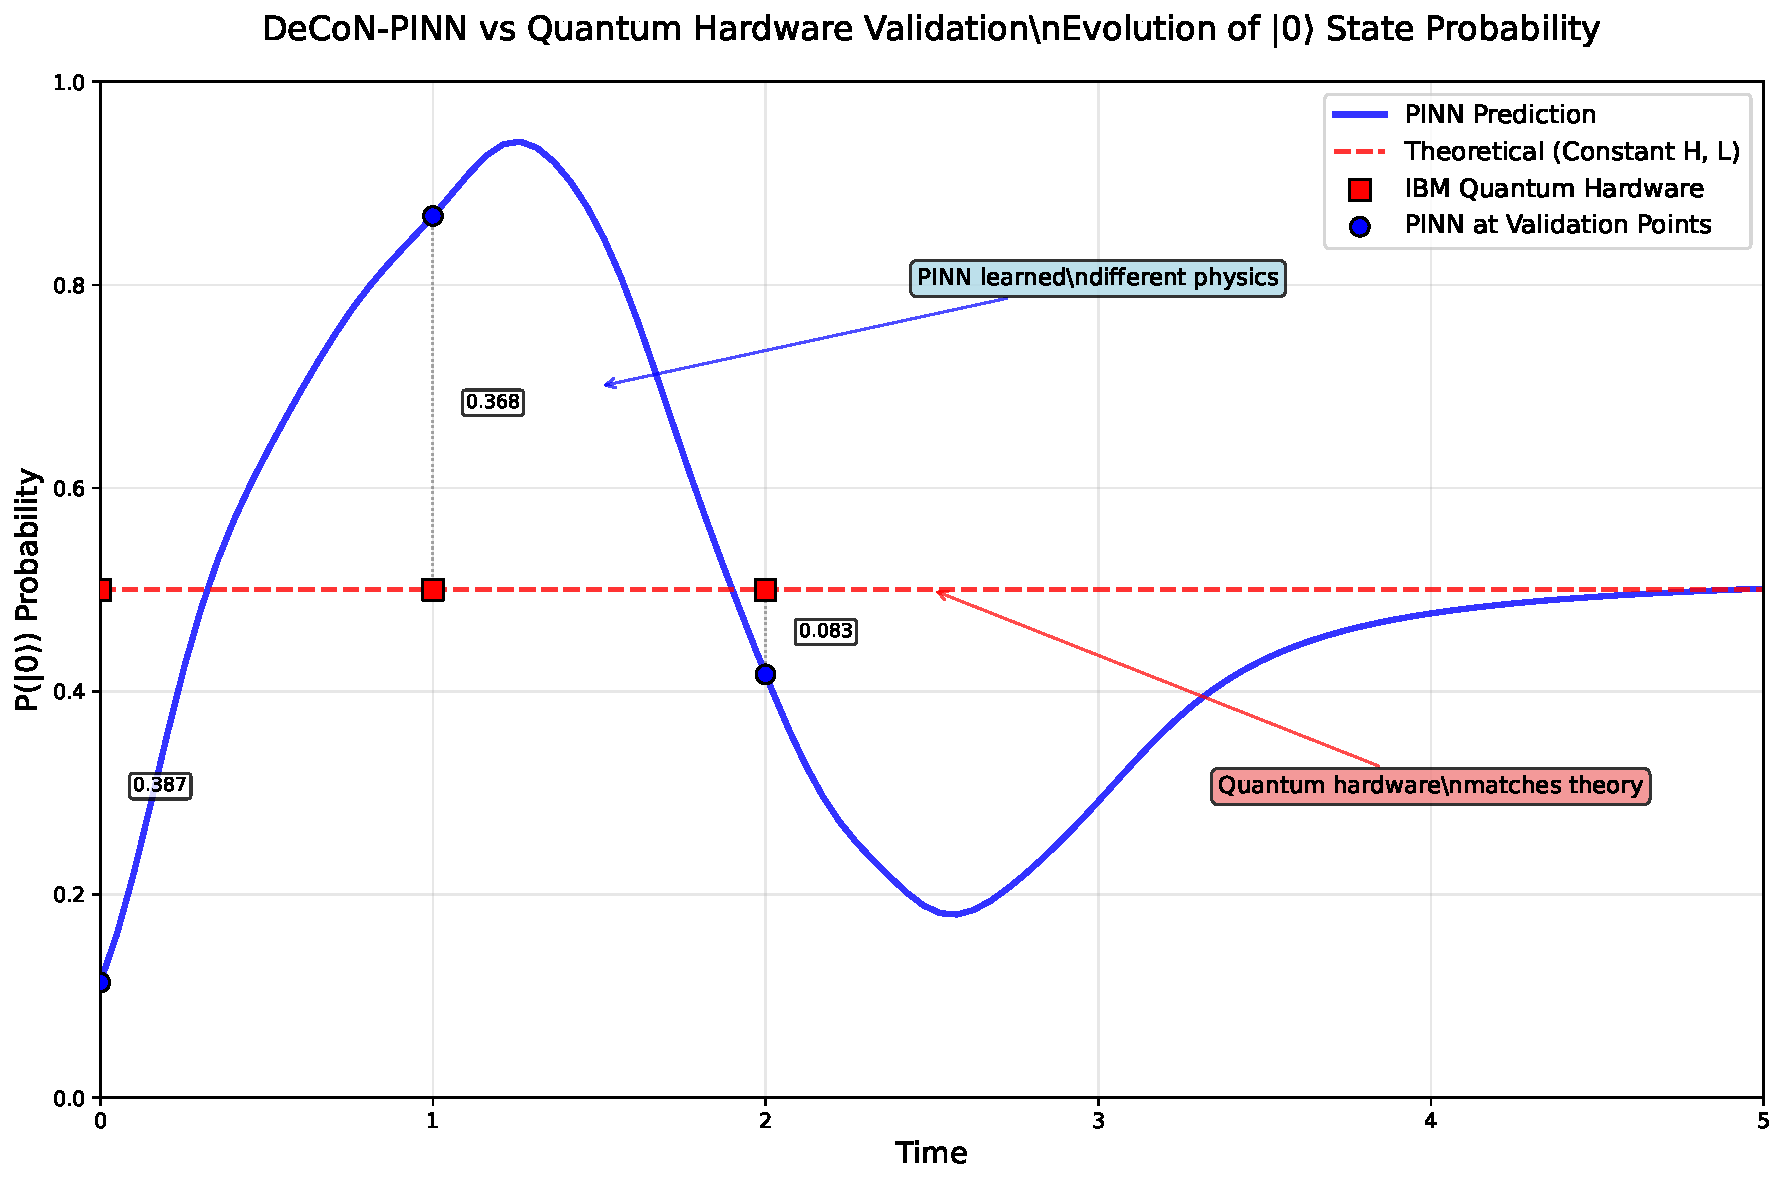
\includegraphics[width=0.75\textwidth]{figures/fig_hardware_comparison.pdf}
\caption{Hardware diagnostic comparison. The PINN prediction varies in time while hardware measurements remain near the stationary expectation for the maximally mixed state.}
\label{fig:hardware-comparison}
\end{figure}

\begin{figure}[H]
\centering
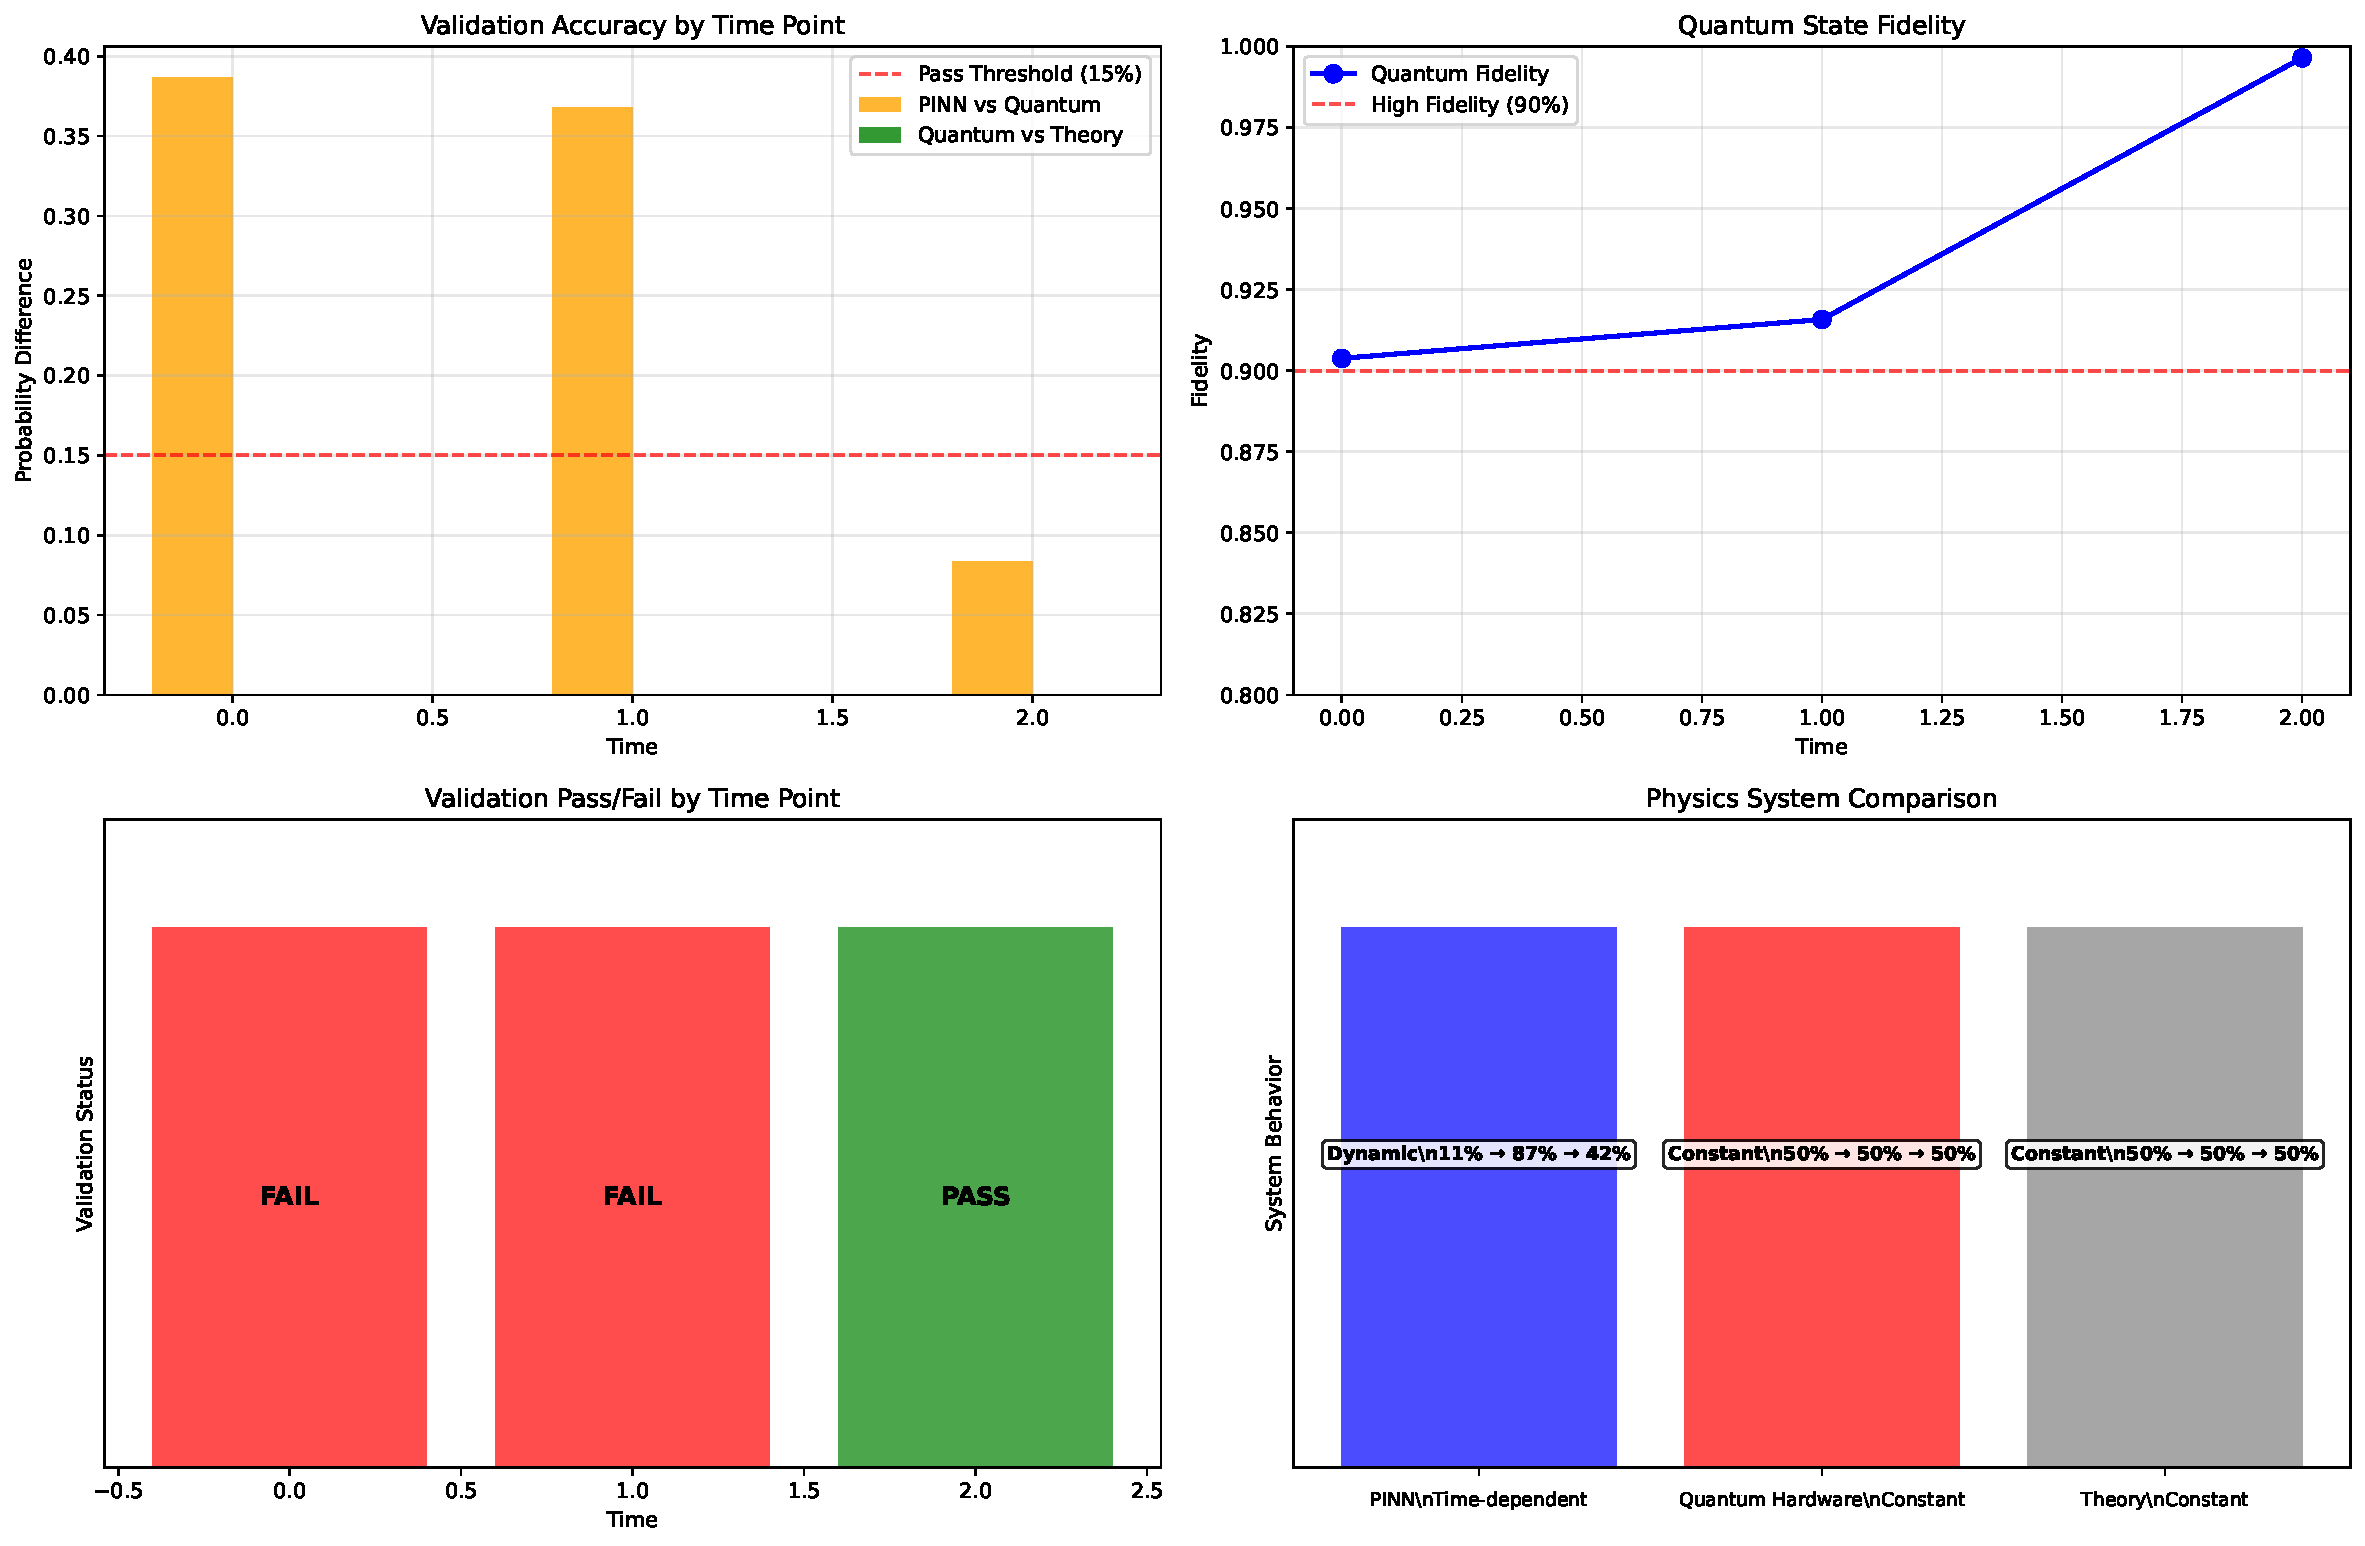
\includegraphics[width=0.75\textwidth]{figures/fig_hardware_metrics.pdf}
\caption{Hardware validation metrics summarizing probability differences and fidelity by validation time point.}
\label{fig:hardware-metrics}
\end{figure}

\section{Discussion}

The central result of this work is architectural rather than purely numerical.
By parameterizing the density matrix as a trace-normalized Gram matrix, the network output is restricted to the physically admissible state manifold throughout training and evaluation.
This differs fundamentally from penalty-based PINNs, where Hermiticity, trace normalization, and positivity remain soft objectives that can be violated during optimization even when the final loss is small.
In this sense, the present approach removes an entire class of failure modes rather than merely reducing their frequency.

This perspective is consistent with a broader view emerging in the PINN literature: many training pathologies are not solely optimizer issues, but reflect a mismatch between the geometry of the target solution space and the parameterization used to represent it \cite{wang2020gradient,jiang2025deeperpinns}.
The spectral-bias literature suggests that gradient-based networks preferentially learn low-frequency or overly smooth components first, which can encourage trivial or nearly stationary solutions in physics-constrained settings \cite{rahaman2019,xu2018,arpit2017,neyshabur2014,zhang2017}.
Our results support that interpretation.
The penalty-based baseline is more vulnerable to unphysical trajectories and fixed-point-like behavior, whereas the constraint-preserving PINN preserves validity by construction and therefore narrows the space of admissible failure modes.

The significance of the method is also not limited to the single dephasing example emphasized in the main text.
As reflected in the comparative analyses reported above, the same architectural idea remains compatible with qualitatively different training regimes and evaluation settings, including frequency-domain diagnostics, gradient-pathology analysis, and depth-dependent refinement studies.
Across these settings, the key advantage is not that the constrained model must achieve the lowest trajectory error in every experiment, but that it reliably excludes non-physical outputs.
That distinction matters in quantum applications, where a numerically accurate but non-positive density matrix is not merely imperfect --- it is physically uninterpretable.

The hardware study should be understood in this same architectural framework.
Its main value is diagnostic, not celebratory.
The disagreement between PINN predictions and IBM hardware did not invalidate the constraint-preserving PINN; instead, it exposed a mismatch between the modeled initial condition and the state preparation implemented on hardware, and clarified the role of stationary states in Lindblad dynamics.
This is an important methodological point: hardware comparisons can reveal hidden inconsistencies in modeling assumptions even when they do not yet constitute a full end-to-end validation of non-trivial learned dynamics.

Several limitations remain.
The present paper is still fundamentally a one-qubit study, and extension to multi-qubit systems will require generalized initial-condition enforcement and more demanding optimization.
Likewise, while the hardware pipeline is useful as a consistency check, direct hardware validation of the IC-enforced non-trivial dynamics remains future work.
The broader implication is therefore best stated carefully: constraint-preserving architectures provide a robust foundation for quantum PINNs, and hardware-aware diagnostics provide a practical way to stress-test the physical assumptions built into those models.

\section{Conclusion}

We introduced a constraint-preserving PINN architecture that guarantees valid quantum density matrices by construction, replacing soft constraint penalties with an explicit representation of the physical state manifold.

Across repeated trials and comparative analyses, the main benefit of this approach is not simply improved stability, but the exclusion of non-physical outputs that remain possible in penalty-based baselines.

We further showed that quantum hardware comparison can serve as a diagnostic tool: rather than merely confirming agreement, it can expose hidden inconsistencies in initial conditions and dynamical assumptions.

Taken together, these results position constraint-preserving PINNs as a robust foundation for reliable open-system modeling and for future hardware-aware validation workflows.

\section*{Appendix: Spectral Bias Supplement}

\begin{figure}[H]
\centering
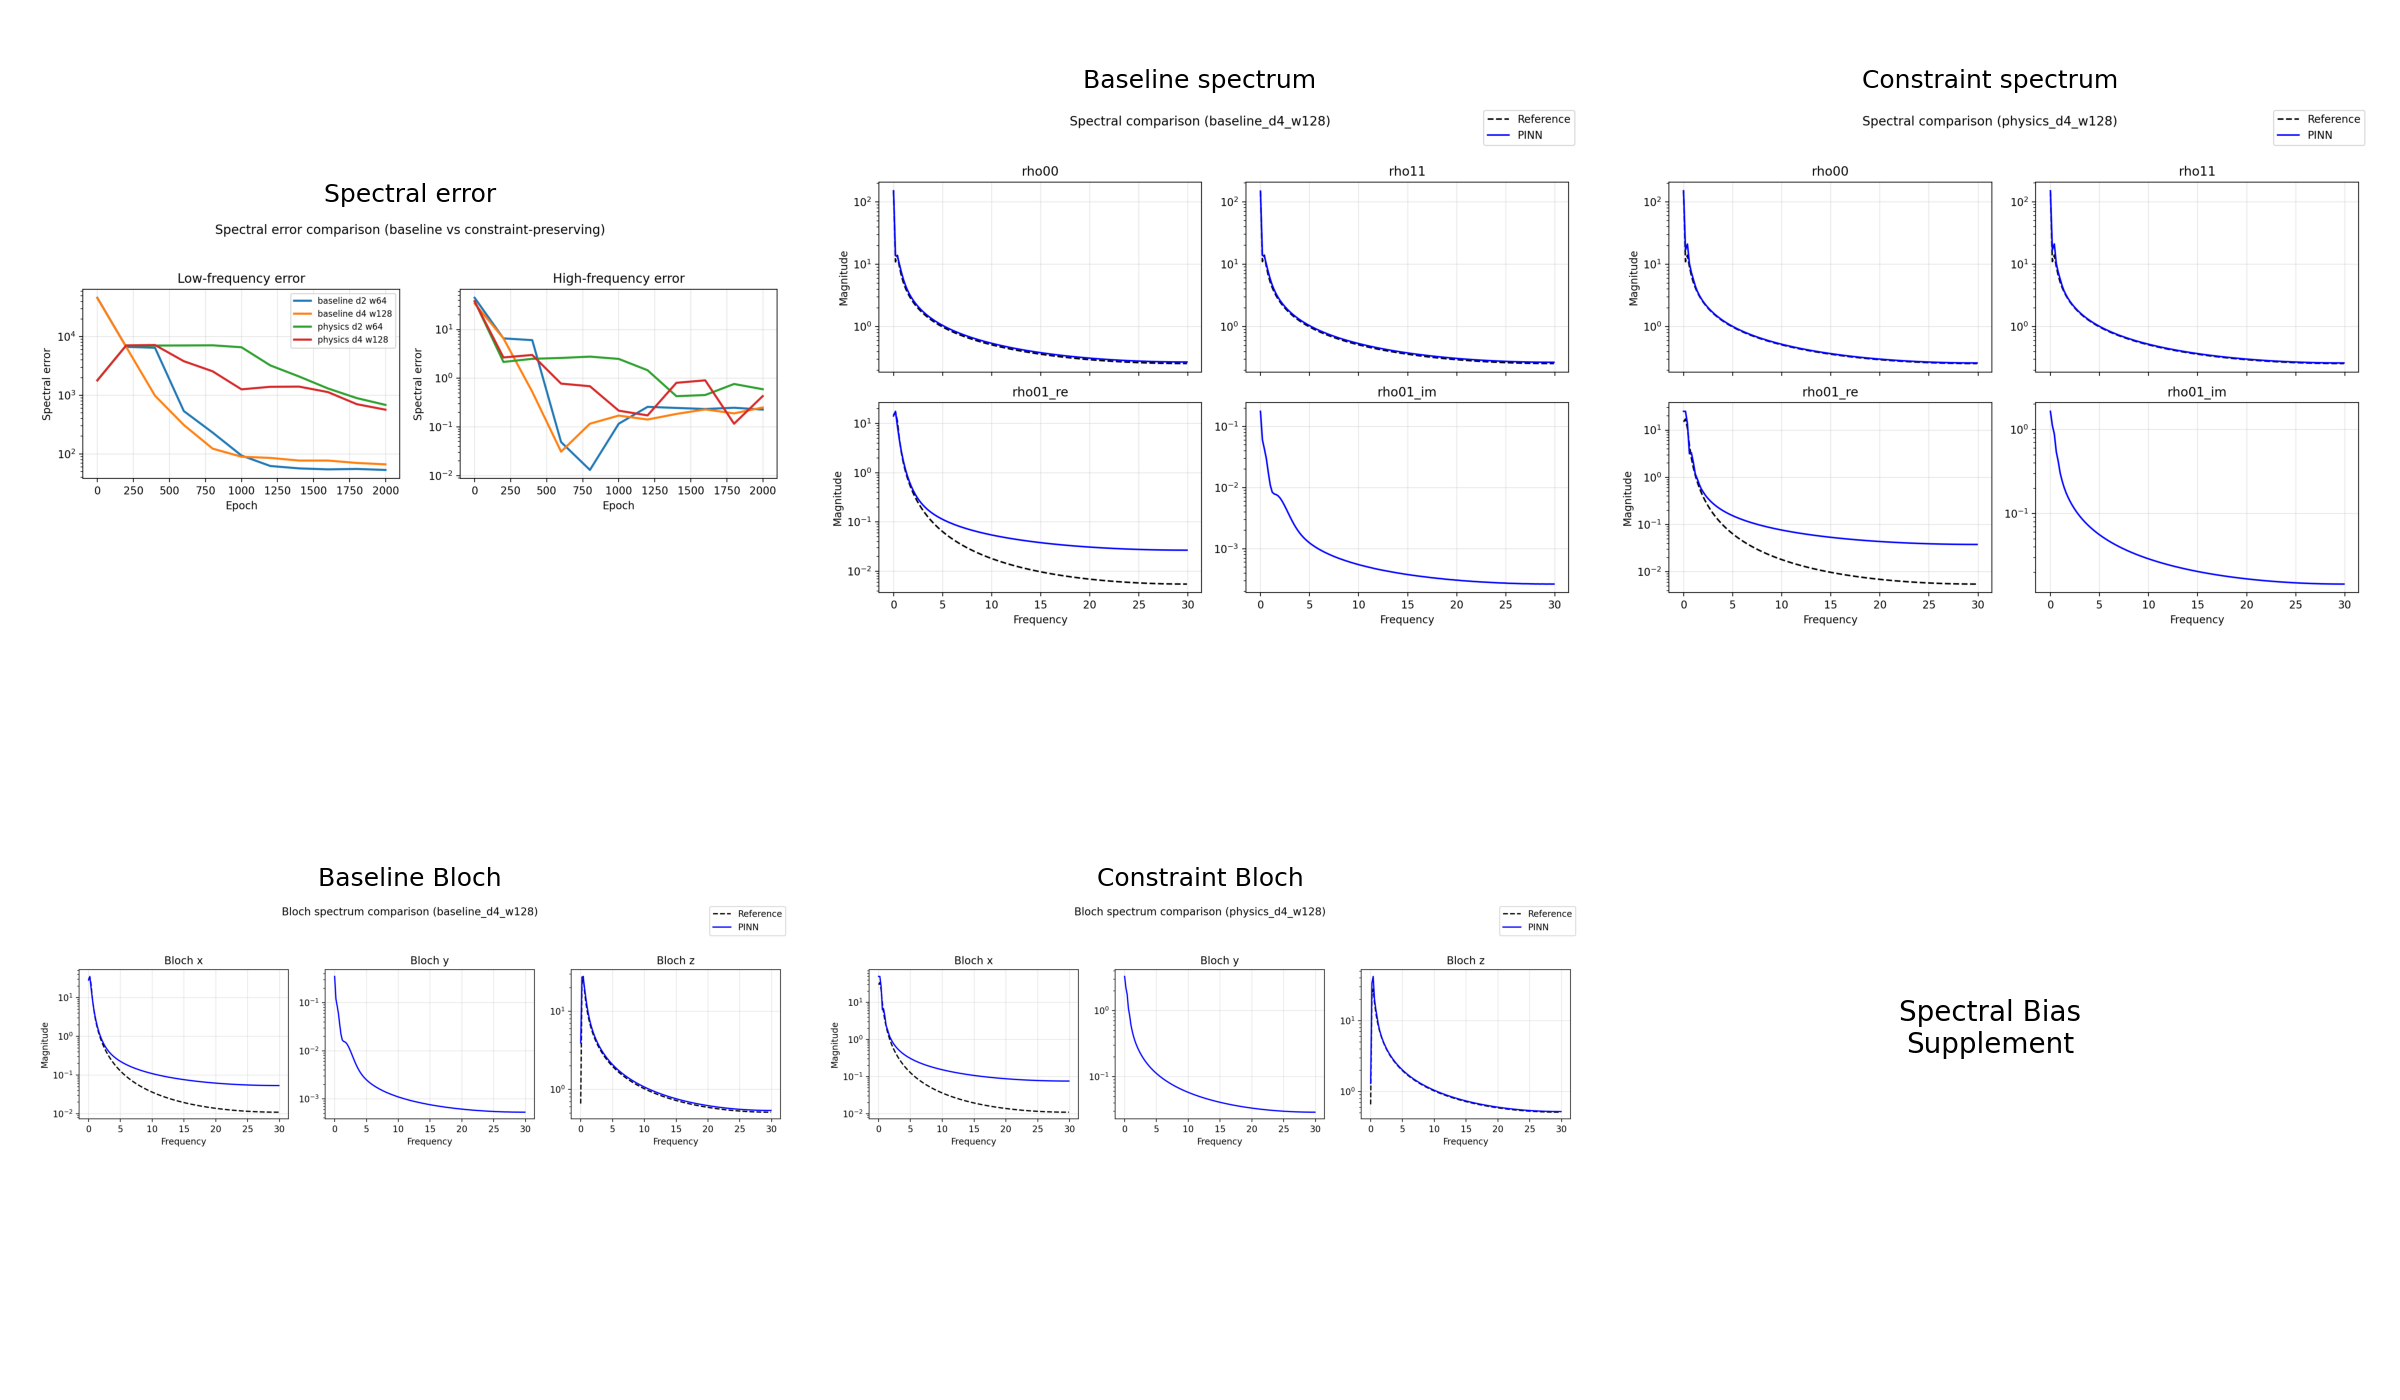
\includegraphics[width=\linewidth]{figures/spectral_bias/spectral_bias_appendix_grid.png}
\caption{Supplemental spectral-bias panels. Top row: spectral error trajectories and final spectra comparisons. Bottom row: Bloch-vector spectra for baseline and constraint-preserving models.}
\label{fig:spectral_appendix}
\end{figure}

\newpage
\bibliographystyle{plain}
\bibliography{references}


\end{document}
